\documentclass[handout]{beamer} % [handout] para imprimir eliminando transiciones

%\usefonttheme[onlymath]{serif}
%\usepackage{fontspec}
%\defaultfontfeatures{Mapping=tex-text}
%\setsansfont[Ligatures={Common}]{Futura}
%\setmonofont[Scale=0.8]{Monaco}

\usepackage{beamerthemesplit}
\usepackage[utf8]{inputenc}
\usepackage[spanish]{babel}
\mode<presentation>
\usetheme{default}
\usecolortheme{dolphin}
\usepackage{alltt}    % \begin{alltt}
\usepackage{amssymb}  % mathematical symbols
\usepackage{comment}
\usepackage{multicol} % \multicols
\usepackage{multirow} % \multirows
\usepackage{tabto}    % \tabto
\usepackage{verbatim} % comentarios

\title{Estructuras de datos}   %[titulo corto]
\author{Fabián Riquelme Csori} %[nombre corto]
\date{2017}                    %[fecha corta]
\institute{Universidad de Valparaíso}                 %[instituto corto]

\newcommand{\HRule}{\rule{\linewidth}{0.2mm}\\[1ex]}
\newcommand{\blue}[1]{\textcolor{blue}{#1}}
\newcommand{\red}[1]{\textcolor{red}{#1}}
\newcommand{\redb}[1]{{\color{red!70!black}{#1}}}
\newcommand{\green}[1]{{\color{green!70!black}{#1}}}
\newcommand{\gray}[1]{{\color{gray!50!white}{#1}}}
\newcommand{\textgreek}[1]{\begingroup\fontencoding{LGR}\selectfont#1\endgroup}
% \alert{texto destacado en rojo}
% \color{green} Color en verde
% \structure{texto en lila}

\begin{document}


%\begin{frame}%[plain]
%  \titlepage
%\end{frame}
%
% [opciones]:
% plain: oculta barra de navegacion, deja + espacio para contenido
% fragile: usar comandos como verbatim
% b,c,t: alineacion vertical
% label=nombre_etiqueta
% allowframebreaks: divide contenido en varios frames si es demasiado largo
% shrink: para escribir mucho texto en una transparencia, reduciendo tamano de fuente

%%%%%%%%%% PORTADA %%%%%%%%%%
\begin{frame}[plain]
  \begin{figure}[h]
    \begin{minipage}{0.3\textwidth}
    
\includegraphics[width=.9\textwidth]{./image/logo-UV.png}
    \end{minipage}
    \begin{minipage}{0.65\textwidth}
     $~$\\[3.6ex]
     \footnotesize{Escuela de Ingeniería Civil Informática}\\
     \footnotesize{Facultad de Ingeniería}
    \end{minipage}
  \end{figure}
  \begin{center}
    \vspace{1ex}
    \HRule
    \Large{Estructuras de datos}\\{\small Capítulo IV: Hashing}\\[-1ex]
    \HRule\vspace{1ex}
    \large{Fabián Riquelme Csori}\\[.5ex]\footnotesize{fabian.riquelme@uv.cl}\\[6ex] {\tiny 2017-II}\\[6ex]
  \end{center}
\end{frame}

%%%%%%%%%% INDEX %%%%%%%%%%
\begin{frame}
 \frametitle{Index}
 \scriptsize 			% reducir tamano de letra
 \tableofcontents		%[pausesections]
\end{frame}

%%%%%%%%%%% ACTUAL INDEX %%%%%%%%%%
%\AtBeginSection[] %generar indice automaticamente
%{
%\begin{frame}<beamer>%[plain]
% \frametitle{Index}
% \framesubtitle{subtitulo}
% \scriptsize
% \tableofcontents[currentsection, currentsubsection]
%\end{frame}
%}

%==============================
\section{Tablas Hash}

%-----------------------
\subsection{Preliminares}

\begin{frame}{Arreglo asociativo}
    \scriptsize{
    \begin{tabular}{lp{60ex}}\hline\\[-1ex]
      {\bf\normalsize associative array} & Collection of \blue{(key, value)} pairs, such that each possible key appears at most once in the collection.\\
      {\bf\small operations}  & \\
      add(key,value)             & Add a new pair to the collection.\\
      remove(key) & Remove the pair from the collection associated to the key.\\
      reassign(key,value) & Replace the value of an existing pair associated to the key.\\
      lookup(key) & Find the value of the pair associated with a given key.\\[1.5ex]\hline
    \end{tabular}

    \begin{itemize}
        \item<2-> Los arreglos asociativos también se conocen como \blue{vectores asociativos}, \blue{mapas}, \blue{tablas de símbolos} o \blue{diccionarios}.
        \item<3-> Las estructuras de datos más comunes que se implementan para manipularlos son las \blue{\bf tablas hash} y los \blue{árboles de búsqueda}.
    \end{itemize}}
\end{frame}

\begin{frame}{Arreglo asociativo: implementación}
    \begin{center}
    \begin{tabular}{l|l|c|c}
        \multicolumn{2}{l|}{} & \multirow{2}{*}{Hash table} & Self-balancing\\
        \multicolumn{2}{l|}{} & & binary search tree \\\hline
        \multirow{2}{*}{add}  & average & $O(1)$ & $O(\log n)$\\\cline{2-4}
        & worst case & $O(n)$ & $O(\log n)$\\\hline
        \multirow{2}{*}{remove} & average & $O(1)$ & $O(\log n)$\\\cline{2-4}
        & worst case & $O(n)$ & $O(\log n)$\\\hline
        \multirow{2}{*}{lookup} & average & $O(1)$ & $O(\log n)$\\\cline{2-4}
        & worst case & $O(n)$ & $O(\log n)$\\
    \end{tabular}
    \end{center}
\end{frame}

\begin{frame}{Tablas Hash}
    \begin{center}
        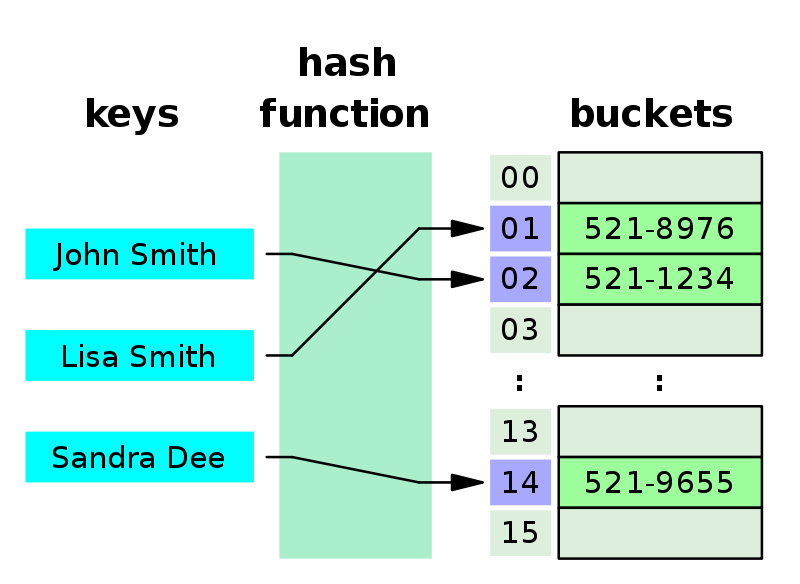
\includegraphics[width=.7\textwidth]{./image/cap4/hash-table.png}\\
        {\tiny [Jorge Stolfi, Wikipedia]}
    \end{center}
    \vspace{-2ex}

    \begin{itemize}
      \item<2-> Si la función de hash es \blue{inyectiva} se habla de \blue{hashing perfecto}.
      \item<3-> Usualmente la tabla hash debe lidiar con \blue{colisiones}.
    \end{itemize}
\end{frame}

\begin{frame}{Tablas Hash: Aplicaciones}
    \begin{itemize}
        \item<1-> El \blue{hashing} se usa para almacenar muchos datos sobre los que se realizarán operaciones de búsqueda e inserción.\\
        {\footnotesize Ej: diccionarios, indexación de BDs, conjuntos, cachés, criptografía, etc.}
        \item<2-> Los datos se almacenan en posiciones pseudo-aleatorias,\\no están ordenados (a diferencia de los árboles), y\\ recorrerlos por orden es lento (e inservible).
        \item<3-> Es una estructura de datos tan usada que varios lenguajes la incluyen como tipos básicos o librerías estándar.
        \item<4-> \blue{\url{http://www.sha1-online.com/}}
    \end{itemize}
\end{frame}

\begin{frame}{Tablas Hash: Estructura}
    \begin{itemize}
        \item Se representa mediante un array con B posiciones (0,...,B-1).
         \begin{itemize}
           \item h(x)= posición dentro de  (0,...,B-1).
         \end{itemize}
        \item El elemento (x,v) se inserta en esta posición
    \end{itemize}

    \begin{center}
        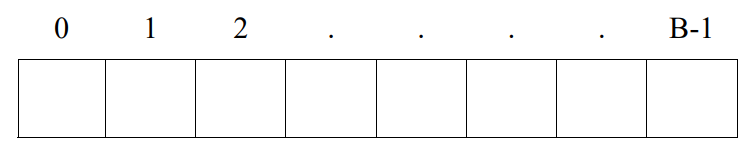
\includegraphics[width=.8\textwidth]{./image/cap4/hassh_array.png}
    \end{center}

\end{frame}

\begin{frame}{Tablas Hash: Estructura}
    \begin{itemize}
        \item Para buscar el elemento con clave x, aplicar la funcon h(x) y buscar la posición correspondiente. Ejemplo
         \begin{itemize}
           \item Si x es de tipo entero \Rightarrow h(x) = x Módulo B \\
           \item Si x es de dipo cadena (string) \Rightarrow  h(x) =  (\displaystyle\sum_{i=1}^{n} ascii (x_i)) Módulo B
         \end{itemize}
        \item El elemento (x,v) se inserta en esta posición
    \end{itemize}


\end{frame}
%-----------------------
\subsection{Colisiones}


\begin{frame}{Ejemplo}
    \begin{center}
        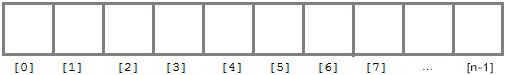
\includegraphics[width=.8\textwidth]{./image/cap4/array.png}
    \end{center}
    \begin{itemize}
        \item<1-> Considere una función de hash tal que \blue{value=table[key\% n]}.
        \begin{itemize}
            \item<2-> Si $n=10$, ¿qué pasa con 143,674 y 645,394?
        \end{itemize}
        \item<3-> Alternativa: suma de dígitos
        \begin{itemize}
            \item<3-> 143,674 = 1 + 4 + 3 + 6 + 7 + 4 = 25
            \item<3-> 645,394 = 6 + 4 + 5 + 3 + 9 + 4 = 31
            \item<4-> ...¿problemas?
        \end{itemize}
        \item<5-> Hashing doble:
        \begin{itemize}
            \item 25 = 2 + 5 = 7
            \item 31 = 3 + 1 = 4
        \end{itemize}
        \item<6-> El problema de \blue{colisiones} se mantiene... ¿soluciones?
    \end{itemize}
\end{frame}

\begin{frame}{Corrección de colisiones: hashing cerrado}
    \begin{itemize}
        \item<1-> \blue{Linear probing}: Si la posición está ocupada, se ocupa la siguiente vacía.
        \item<2-> Ejemplo:\\
        \begin{tabular}{cccc}
        key & hash & index & lin.prob\\\hline
1	& 1 \% 20 = 1	& 1	& 1 \\
2	& 2 \% 20 = 2	& 2	& 2 \\
42	& \hspace{-2ex} 42 \% 20 = 2	& 2	& 3 \\
4	& 4 \% 20 = 4	& 4	& 4 \\
12	& 12 \% 20 = 12	& 12 & 12 \\
14	& 14 \% 20 = 14	& 14 & 14 \\
17	& 17 \% 20 = 17	& 17 & 17 \\
13	& 13 \% 20 = 13	& 13 & 13 \\
37	& 37 \% 20 = 17	& 17 & 18 \\
        \end{tabular}
        \item<3-> ¿Problemas? \uncover<4->{Arruina la eficiencia: $O(1)\to O(n)$}
        \item<5-> Variaciones: \blue{quadratic overflow}, etc.
    \end{itemize}
\end{frame}

\begin{frame}{Corrección de colisiones: hashing abierto}
    \begin{center}
        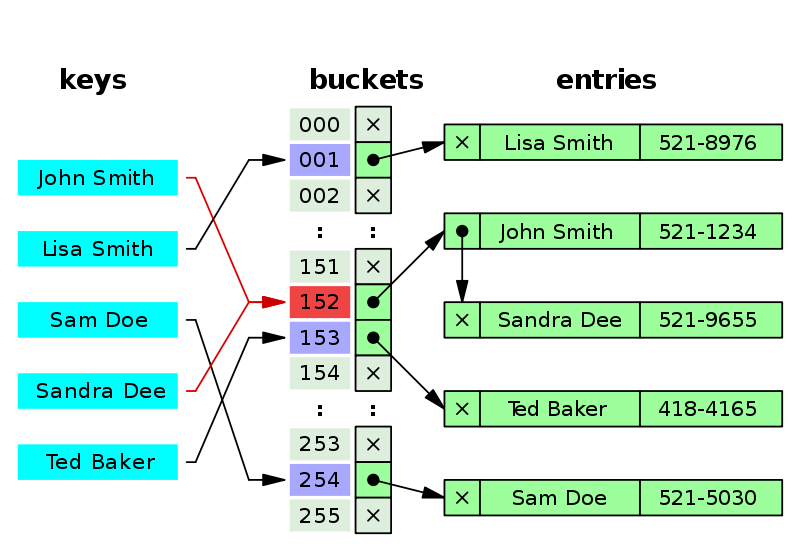
\includegraphics[width=.9\textwidth]{./image/cap4/hash-table-list.png}\\
        Uso de \blue{listas enlazadas} \hspace{15ex} {\tiny [Jorge Stolfi, Wikipedia]}
    \end{center}
\end{frame}

\begin{frame}{Buenas prácticas}
    \begin{block}{Función de hash}
    \begin{itemize}
        \item Debe ser lo más simple posible: $O(1)$
        \item Para un gran número de claves, debe disponer los valores lo más distantes posible.
    \end{itemize}
    \end{block}
    \pause
    \begin{block}{Tabla de hash}
    \begin{itemize}
        \item Si es muy pequeña, aumentará el número de colisiones.
        \begin{itemize}
            \item o bien el uso de listas enlazadas aumentará la complejidad.
        \end{itemize}
        \item Si es muy grande, aumentará innecesariamente el uso de memoria.
    \end{itemize}
    \end{block}
    \pause
    Buenas alternativas son las llamadas \blue{funciones hash criptográficas}.
\end{frame}

\subsection{Analisis} {Ventajas/Desventajas}
\begin{frame}{Ventajas}
\begin{itemize}
  \item No necesita almacenamiento adicional (índice).
  \item Facilita la inserción y eliminación rápida de registros.
  \item Encuentra  registros con muy pocos accesos en promedio al disco.
  \item La idea general de hashing es colocar, en la forma menos relacionada porsible la información facilitando la eficiencia en el acceso.
\end{itemize}
\end{frame}

\begin{frame}{Desventajas}
\begin{itemize}
  \item No se pueden usar registros de longitud variable.
  \item No se pueden aplicar oordenamientos a la información contenida dentro de la tabla.
  \item No permite llaves duplicadas.
\end{itemize}
\end{frame}

\subsection{Ejemplos} {Ejercicios (1)}
\begin{frame}{Ejercicios 1 - Lineal}
\uncover<3>{
\begin{center}
    %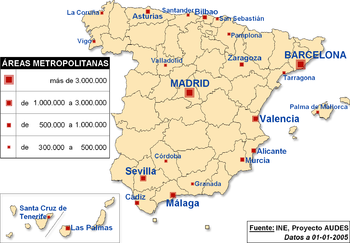
\includegraphics[width=.45\textwidth]{./image/cap3/Mapa_Espana1}
    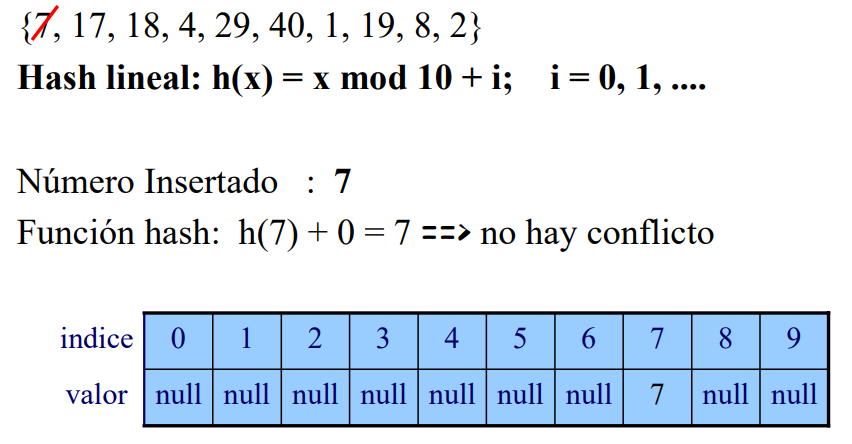
\includegraphics[width=0.7\textwidth]{./image/cap4/hash_01}
\end{center}
}
\end{frame}

\begin{frame}{Ejercicios 1 - Lineal}
\uncover<3>{
\begin{center}
    %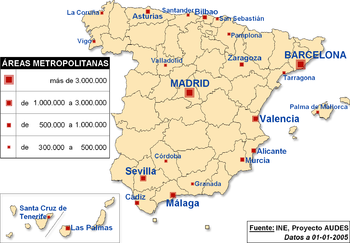
\includegraphics[width=.45\textwidth]{./image/cap3/Mapa_Espana1}
    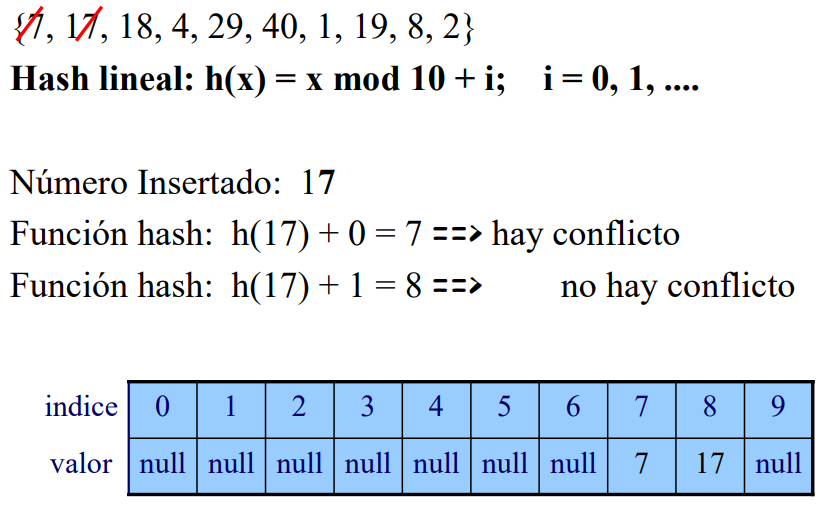
\includegraphics[width=0.7\textwidth]{./image/cap4/hash_02}
\end{center}
}
\end{frame}

\begin{frame}{Ejercicios 1 - Lineal}
\uncover<3>{
\begin{center}
    %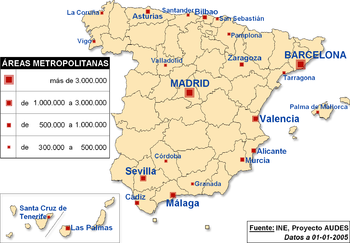
\includegraphics[width=.45\textwidth]{./image/cap3/Mapa_Espana1}
    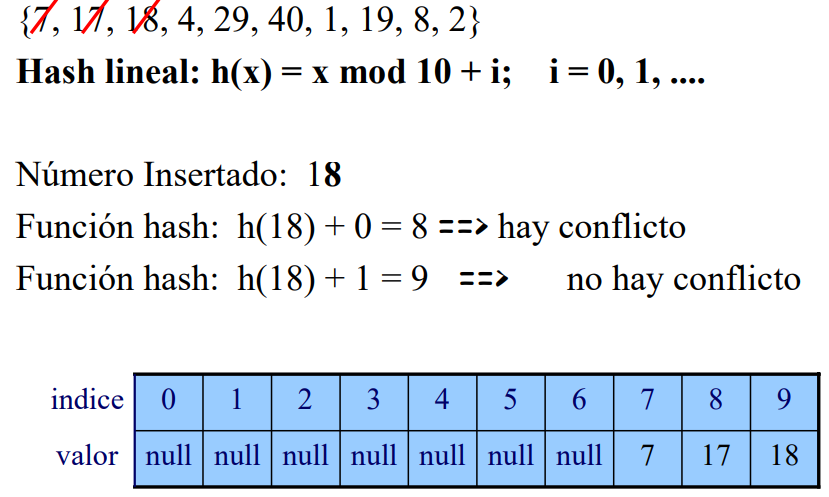
\includegraphics[width=0.7\textwidth]{./image/cap4/hash_03}
\end{center}
}
\end{frame}

\begin{frame}{Ejercicios 1 - Lineal}
\uncover<3>{
\begin{center}
    %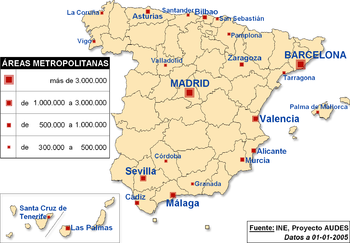
\includegraphics[width=.45\textwidth]{./image/cap3/Mapa_Espana1}
    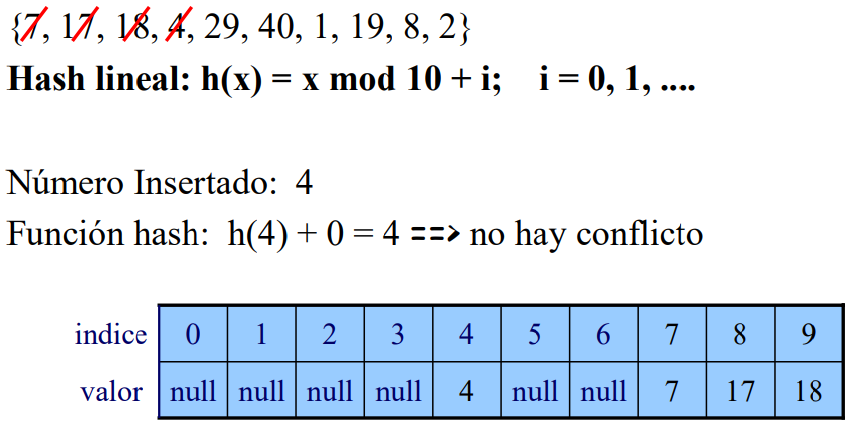
\includegraphics[width=0.7\textwidth]{./image/cap4/hash_04}
\end{center}
}
\end{frame}

\begin{frame}{Ejercicios 1 - Lineal}
\uncover<3>{
\begin{center}
    %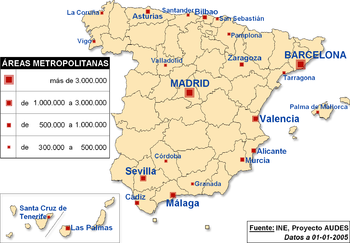
\includegraphics[width=.45\textwidth]{./image/cap3/Mapa_Espana1}
    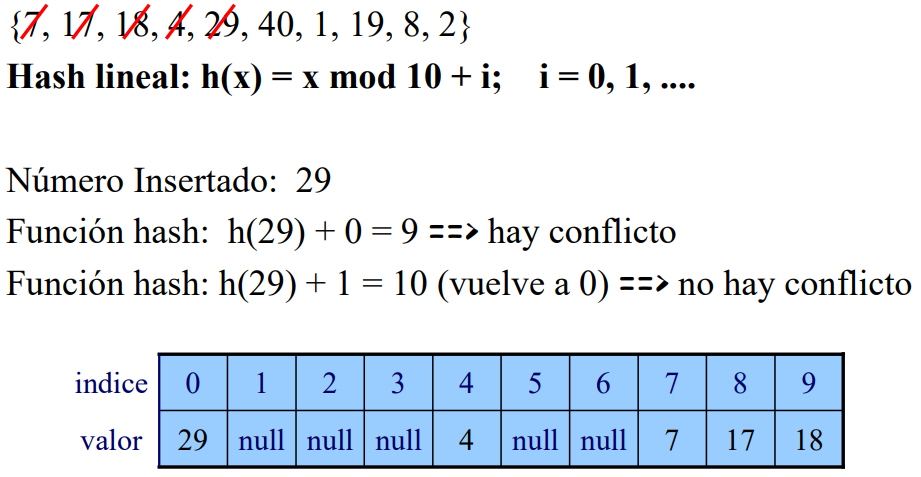
\includegraphics[width=0.7\textwidth]{./image/cap4/hash_05}
\end{center}
}
\end{frame}

\begin{frame}{Ejercicios 1 - Lineal}
\uncover<3>{
\begin{center}
    %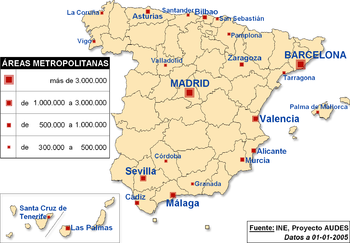
\includegraphics[width=.45\textwidth]{./image/cap3/Mapa_Espana1}
    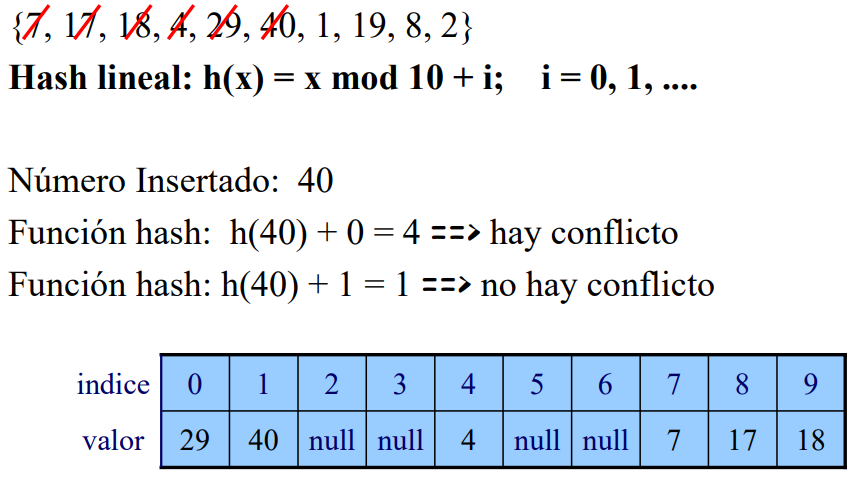
\includegraphics[width=0.7\textwidth]{./image/cap4/hash_06}
\end{center}
}
\end{frame}

\begin{frame}{Ejercicios 1 - Lineal}
\uncover<3>{
\begin{center}
    %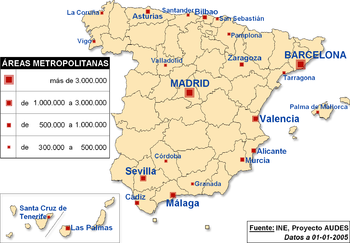
\includegraphics[width=.45\textwidth]{./image/cap3/Mapa_Espana1}
    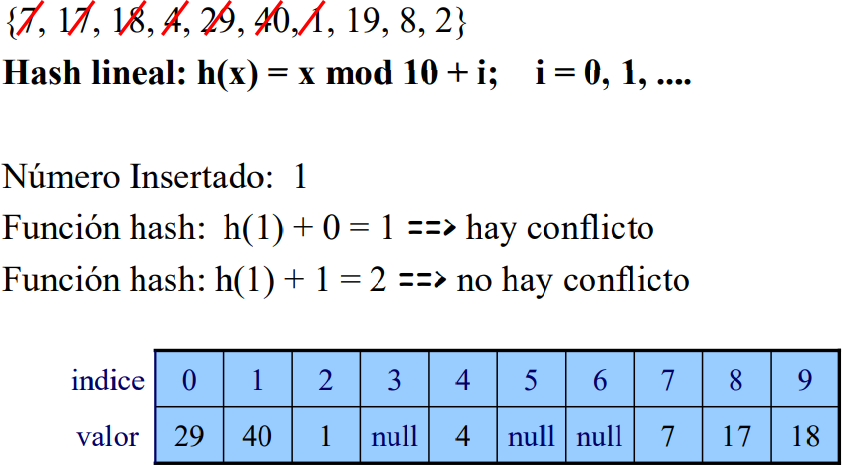
\includegraphics[width=0.7\textwidth]{./image/cap4/hash_07}
\end{center}
}
\end{frame}

\begin{frame}{Ejercicios 1 - Lineal}
\uncover<3>{
\begin{center}
    %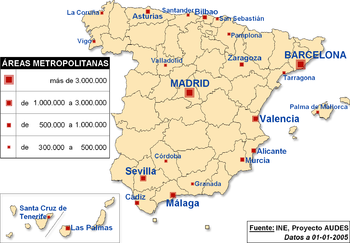
\includegraphics[width=.45\textwidth]{./image/cap3/Mapa_Espana1}
    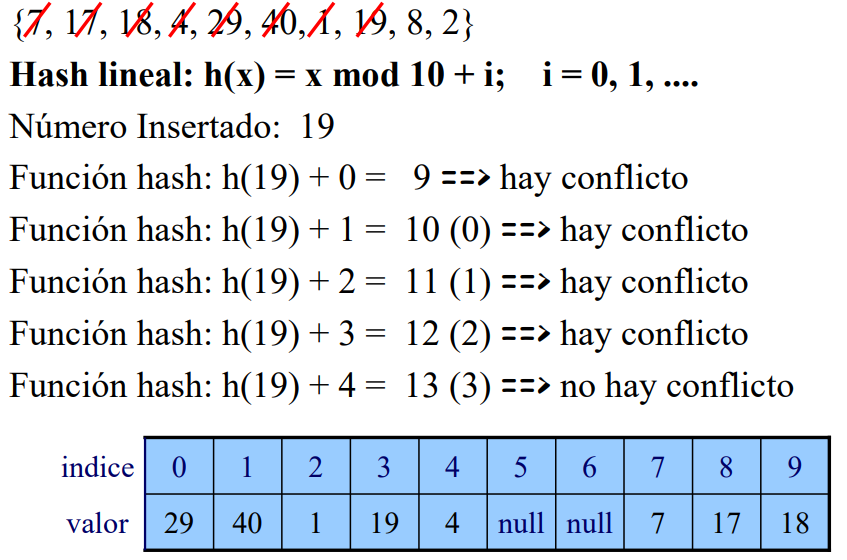
\includegraphics[width=0.7\textwidth]{./image/cap4/hash_08}
\end{center}
}
\end{frame}

\begin{frame}{Ejercicios 1 - Lineal}
\uncover<3>{
\begin{center}
    %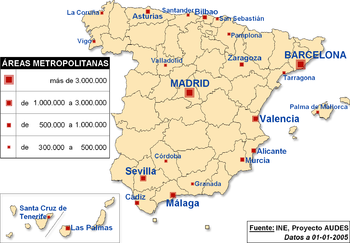
\includegraphics[width=.45\textwidth]{./image/cap3/Mapa_Espana1}
    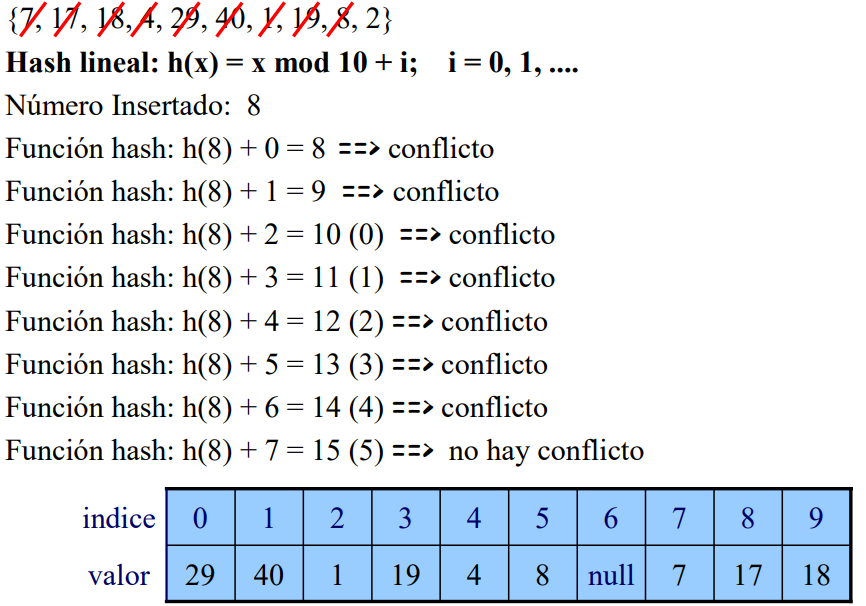
\includegraphics[width=0.7\textwidth]{./image/cap4/hash_09}
\end{center}
}
\end{frame}

\begin{frame}{Ejercicios 1 - Lineal}
\uncover<3>{
\begin{center}
    %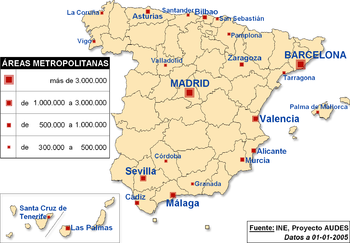
\includegraphics[width=.45\textwidth]{./image/cap3/Mapa_Espana1}
    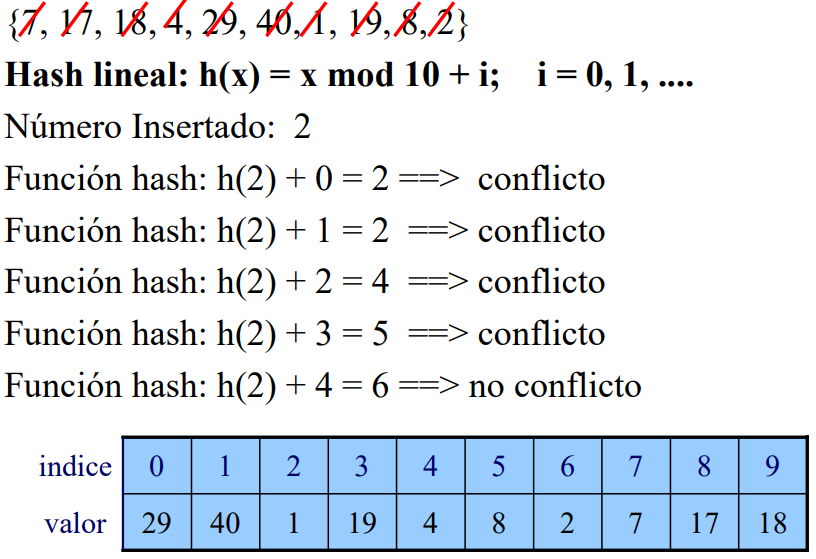
\includegraphics[width=0.7\textwidth]{./image/cap4/hash_10}
\end{center}
}
\end{frame}




\begin{frame}{Ejercicios 2 - Cuadrático}
  \uncover<3>{
  \begin{center}
      %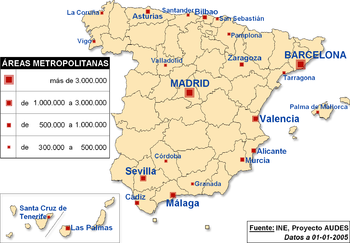
\includegraphics[width=.45\textwidth]{./image/cap3/Mapa_Espana1}
      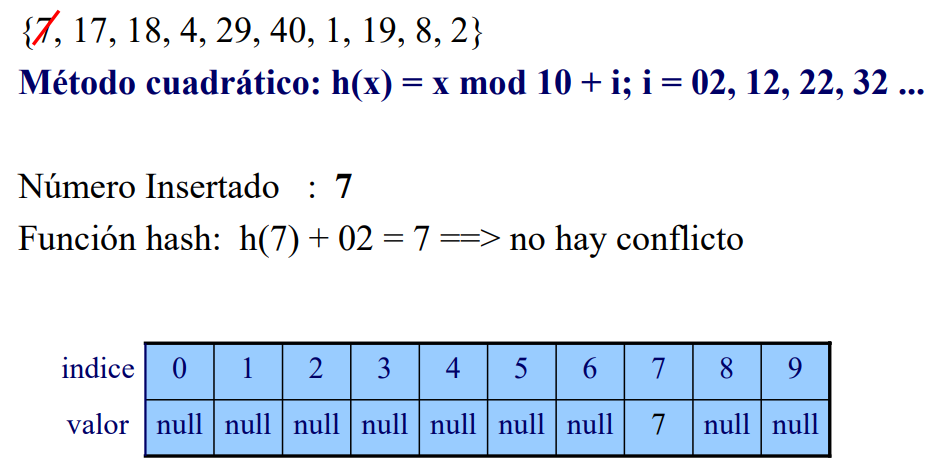
\includegraphics[width=0.7\textwidth]{./image/cap4/hash_11}
  \end{center}
  }
  \end{frame}

\begin{frame}{Ejercicios 2 - Cuadrático}
  \uncover<3>{
  \begin{center}
      %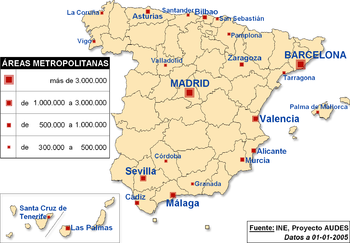
\includegraphics[width=.45\textwidth]{./image/cap3/Mapa_Espana1}
      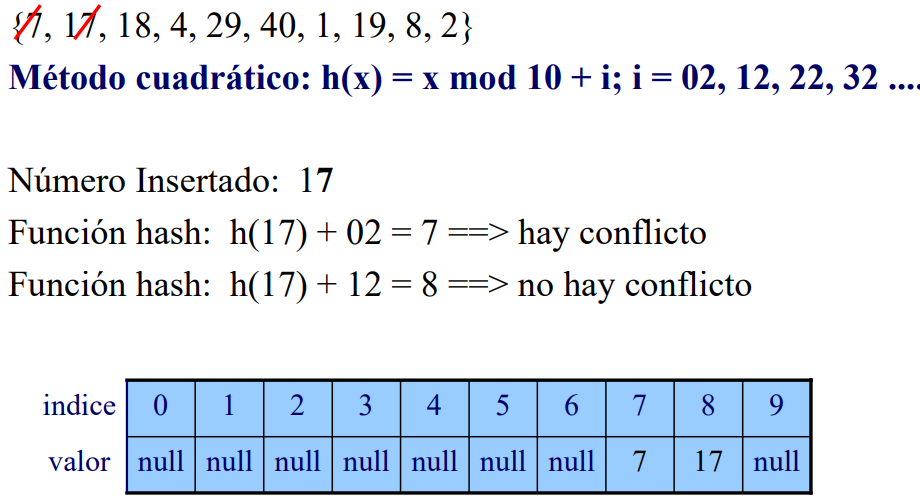
\includegraphics[width=0.7\textwidth]{./image/cap4/hash_12}
  \end{center}
  }
  \end{frame}

  \begin{frame}{Ejercicios 2 - Cuadrático}
  \uncover<3>{
  \begin{center}
      %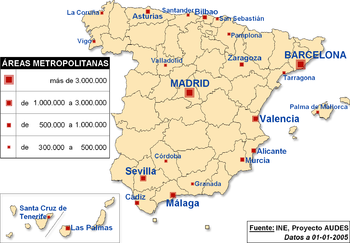
\includegraphics[width=.45\textwidth]{./image/cap3/Mapa_Espana1}
      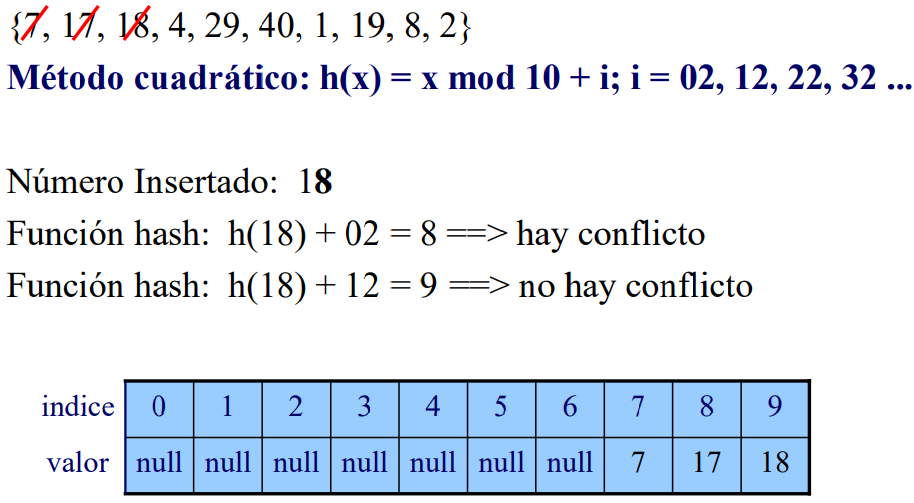
\includegraphics[width=0.7\textwidth]{./image/cap4/hash_13}
  \end{center}
  }
  \end{frame}

  \begin{frame}{Ejercicios 1 - Cuadrático}
  \uncover<3>{
  \begin{center}
      %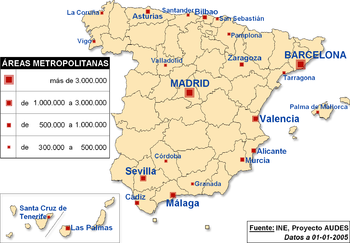
\includegraphics[width=.45\textwidth]{./image/cap3/Mapa_Espana1}
      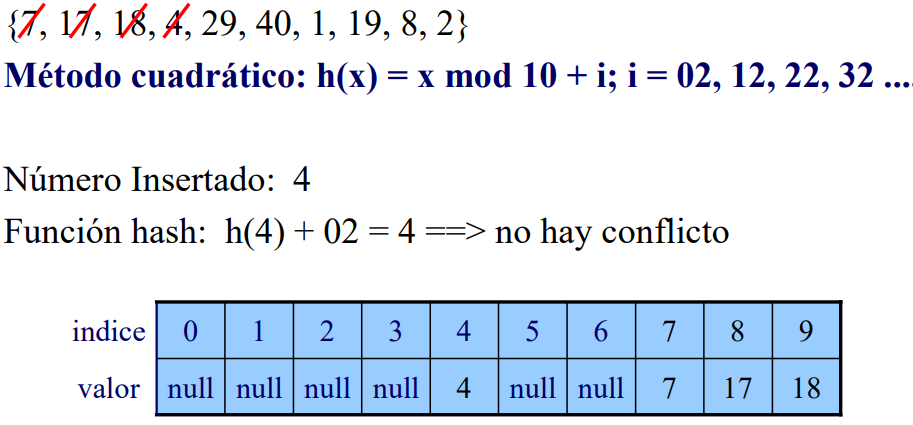
\includegraphics[width=0.7\textwidth]{./image/cap4/hash_14}
  \end{center}
  }
  \end{frame}

  \begin{frame}{Ejercicios 2 - Cuadrático}
  \uncover<3>{
  \begin{center}
      %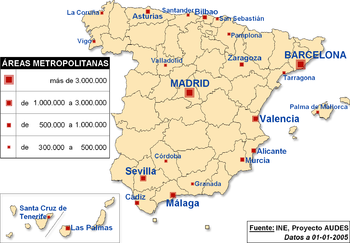
\includegraphics[width=.45\textwidth]{./image/cap3/Mapa_Espana1}
      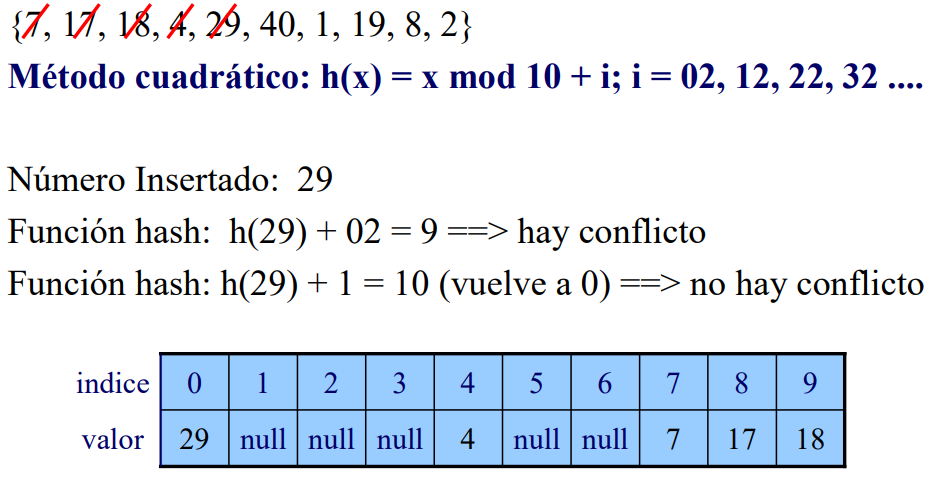
\includegraphics[width=0.7\textwidth]{./image/cap4/hash_15}
  \end{center}
  }
  \end{frame}


  \begin{frame}{Ejercicios 2 - Cuadrático}
  \uncover<3>{
  \begin{center}
      %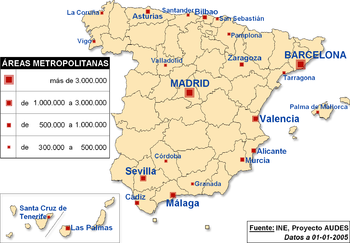
\includegraphics[width=.45\textwidth]{./image/cap3/Mapa_Espana1}
      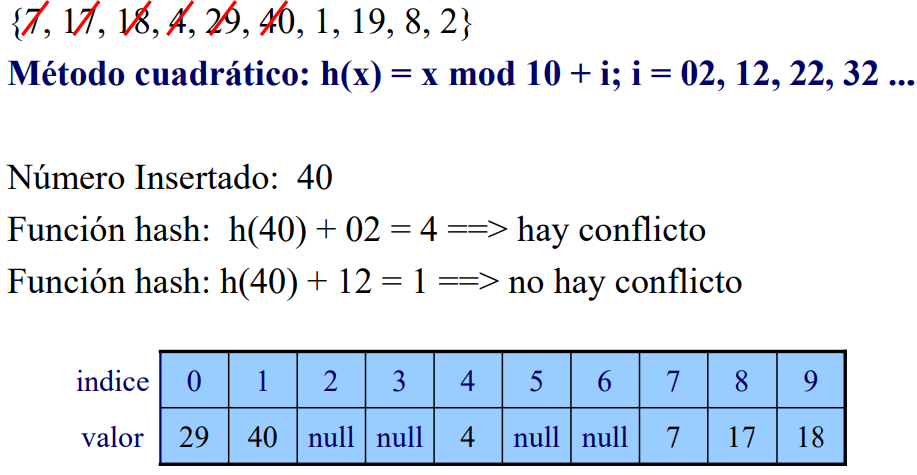
\includegraphics[width=0.7\textwidth]{./image/cap4/hash_16}
  \end{center}
  }
  \end{frame}

  \begin{frame}{Ejercicios 2 - Cuadrático}
  \uncover<3>{
  \begin{center}
      %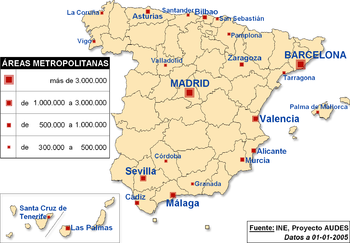
\includegraphics[width=.45\textwidth]{./image/cap3/Mapa_Espana1}
      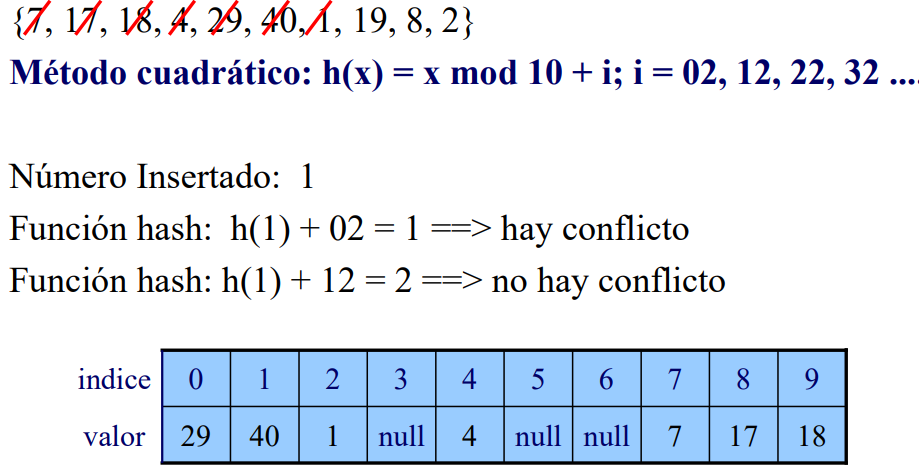
\includegraphics[width=0.7\textwidth]{./image/cap4/hash_17}
  \end{center}
  }
  \end{frame}

  \begin{frame}{Ejercicios 2 - Cuadrático}
  \uncover<3>{
  \begin{center}
      %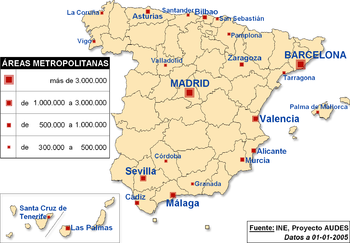
\includegraphics[width=.45\textwidth]{./image/cap3/Mapa_Espana1}
      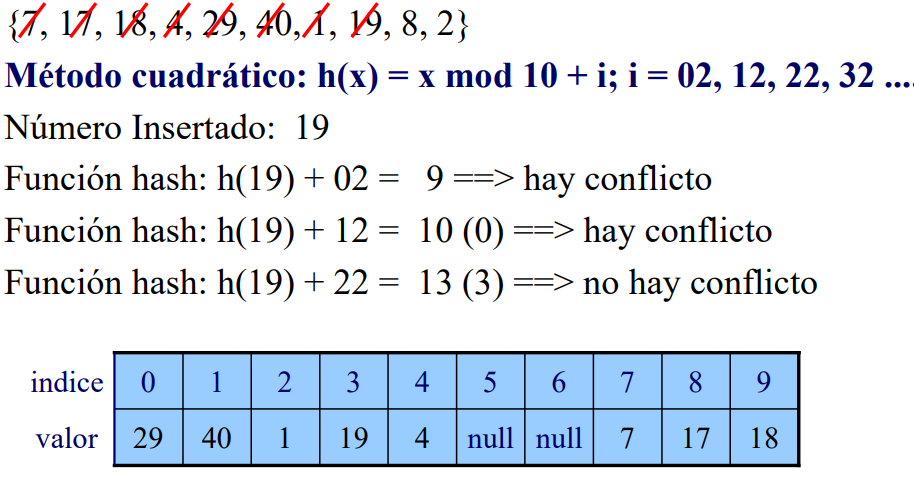
\includegraphics[width=0.7\textwidth]{./image/cap4/hash_18}
  \end{center}
  }
  \end{frame}

  \begin{frame}{Ejercicios 2 - Cuadrático}
  \uncover<3>{
  \begin{center}
      %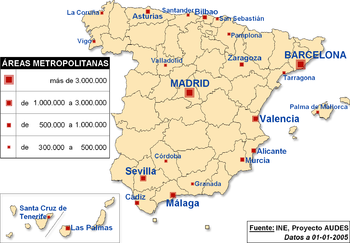
\includegraphics[width=.45\textwidth]{./image/cap3/Mapa_Espana1}
      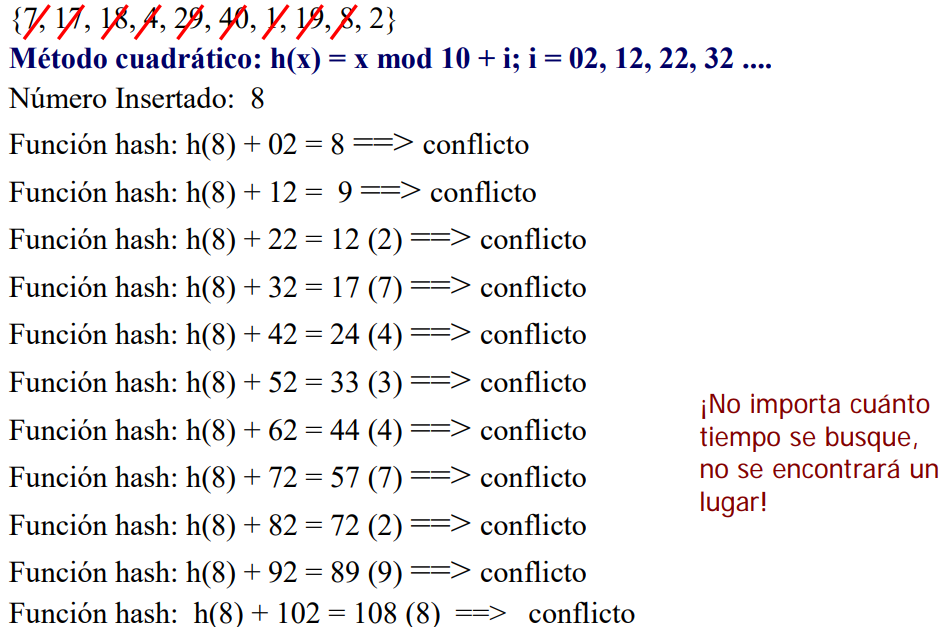
\includegraphics[width=0.7\textwidth]{./image/cap4/hash_19}
  \end{center}
  }
  \end{frame}

  \begin{frame}{Ejercicios 2 - Cuadrático}
  \uncover<3>{
  \begin{center}
      %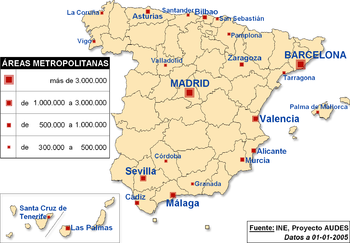
\includegraphics[width=.45\textwidth]{./image/cap3/Mapa_Espana1}
      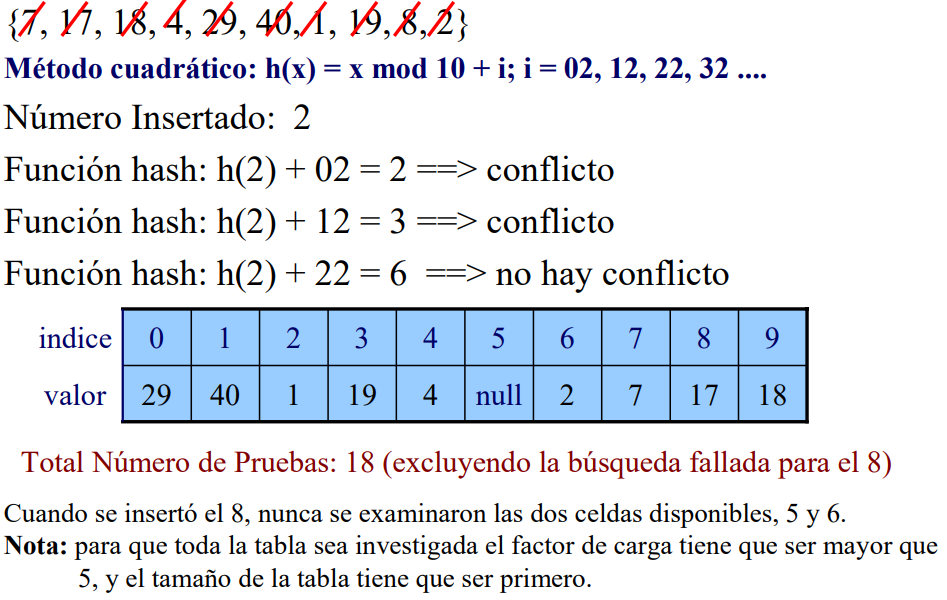
\includegraphics[width=0.7\textwidth]{./image/cap4/hash_20}
  \end{center}
  }
  \end{frame}

  \begin{frame}{Ejercicios 3 - Encadenado}
  \uncover<3>{
  \begin{center}
      %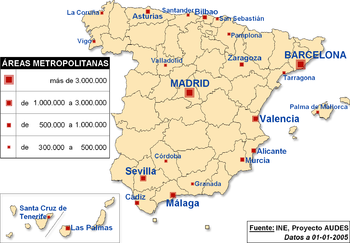
\includegraphics[width=.45\textwidth]{./image/cap3/Mapa_Espana1}
      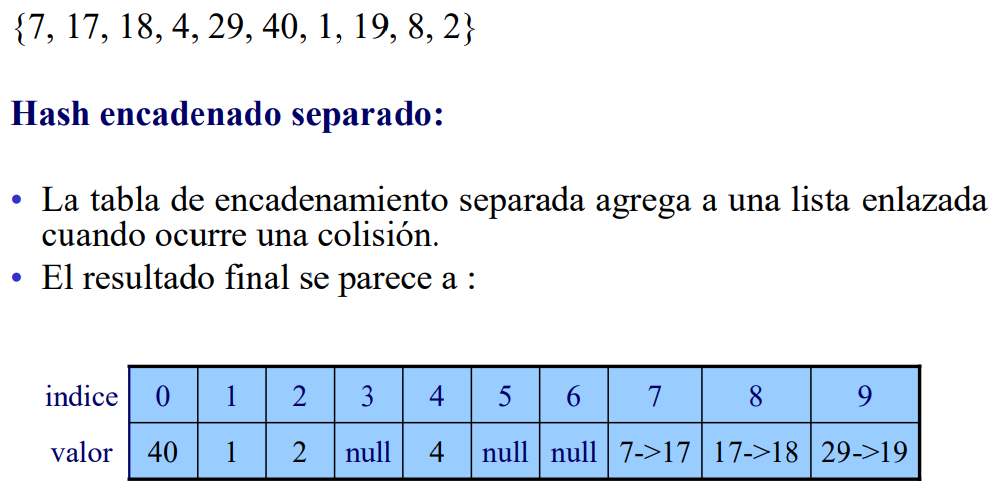
\includegraphics[width=0.7\textwidth]{./image/cap4/hash_21}
  \end{center}
  }
  \end{frame}
%\begin{frame}{Ejercicios (1)}
%    \begin{itemize}
%        \item Busque códigos que implementen una tabla hash
%        \begin{itemize}
%            \item C, C++, Python, Java, otros...
%        \end{itemize}
%        \item Observe los códigos e identifique:
%        \begin{itemize}
%            \item ¿qué función de hash implementan?
%            \item ¿cómo manejan las colisiones?
%        \end{itemize}
%    \end{itemize}
%\end{frame}

\begin{frame}{Ejercicios (2)}

    Dadas las siguientes claves:
    \blue{$$12, 44, 13, 88, 23, 94, 11, 39, 20, 16, 5$$}
    y la función de hash $h(i)=(2i+5)\mbox{mod }11$.

    \begin{itemize}
        \item Dibuje una tabla hash de 11 posiciones de memoria que represente el hashing con un manejo de colisiones usando listas enlazadas.
        \item Repita el ejercicio anterior, pero usando linear probing.
        \item Repita el ejercicio anterior, pero usando quadratic probing.
        \item Implemente cada una de las soluciones.
    \end{itemize}
\end{frame}

\begin{frame}{Ejercicios (3)}

    Busque y responda:

    \begin{itemize}
        \item ¿Qué se entiende por \blue{\em rehashing} y cuando se aplica?
        \item ¿Qué es el \blue{\em load factor}?
        \item Como formas de manejo de colisiones hemos visto {\em linear probing}, {\em quadratic probing} y uso de listas enlazadas.\\
        ¿En qué consiste el \blue{\em double hashing}?
    \end{itemize}
\end{frame}

%------------------------------

\begin{frame}
 \begin{block}{Bibliografía recomendada}
  \begin{itemize}
    \item Weiss, M., Estructura de datos y algoritmos,\\ Addison-Wesley, 1995.
    \item Aho, Hopcroft y Ullman, Estructuras de datos y algoritmos, Addison-Wesley, 1988.
  \end{itemize}
 \end{block}
 \begin{block}{Recursos}
  \begin{itemize}
    \item Wikimedia Commons.
  \end{itemize}
 \end{block}
\end{frame}

\end{document}
